%Architecture
In this section we describe in detail the system architecture, in particular the memory hierarchies along with the data mapping and refresh policies that we adopt.

Figure~\ref{fig:reva} shows the complete PICASSO architecture.

\begin{figure*}[ht!]
\begin{minipage}[b]{0.33\linewidth}
\raggedleft
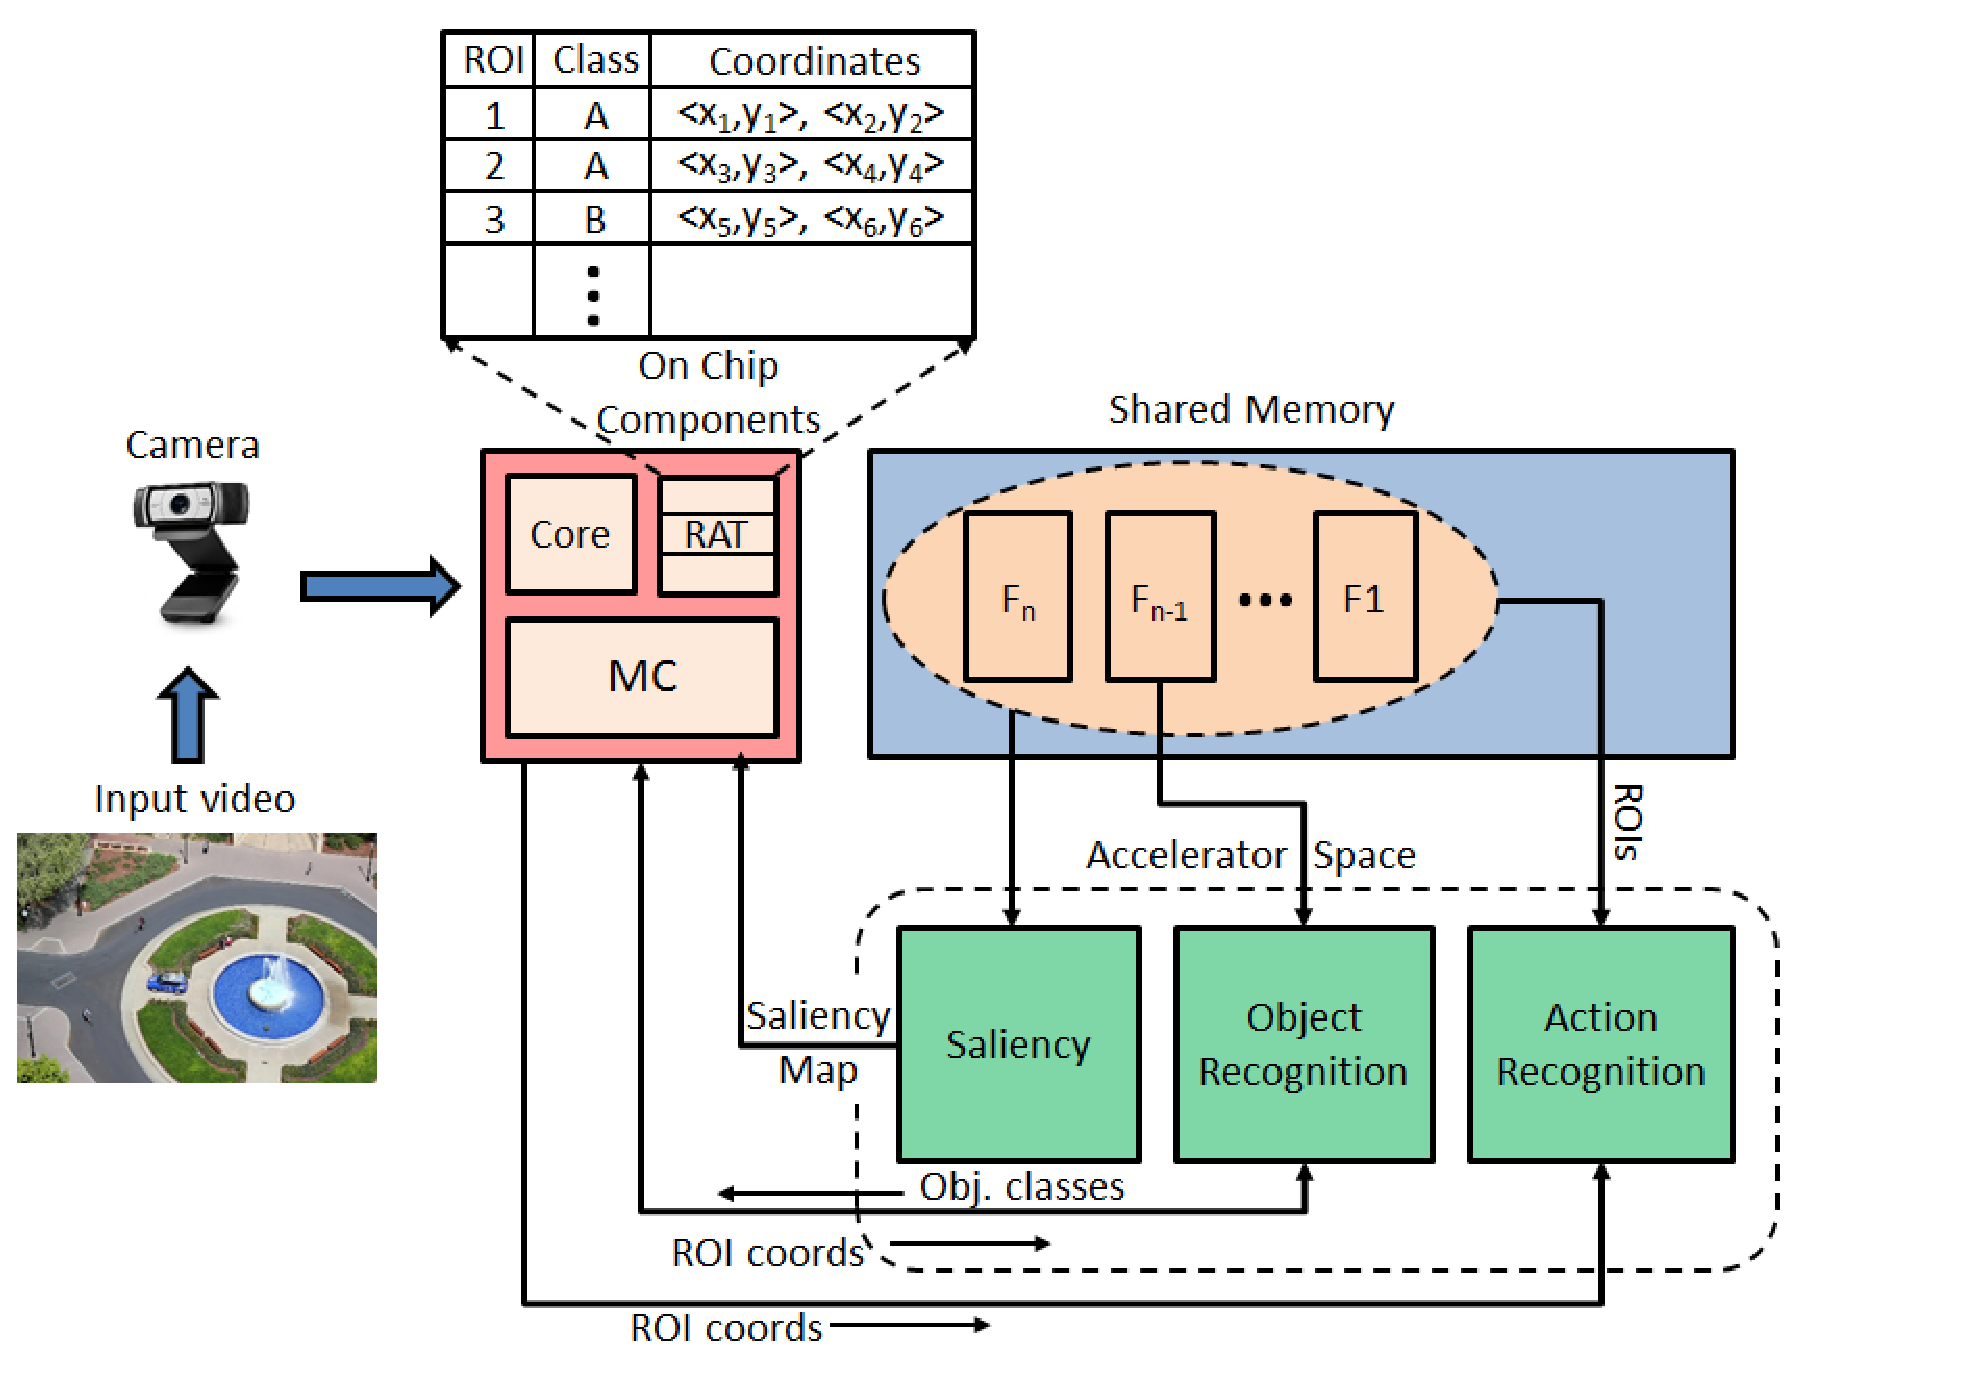
\epsfig{file=figs/baseline_arch.eps, angle=0, width=1\linewidth, clip=}
\caption{\label{fig:reva}a) Architecture of Proposed System}
\end{minipage}
\begin{minipage}[b]{0.35\linewidth}
\centering
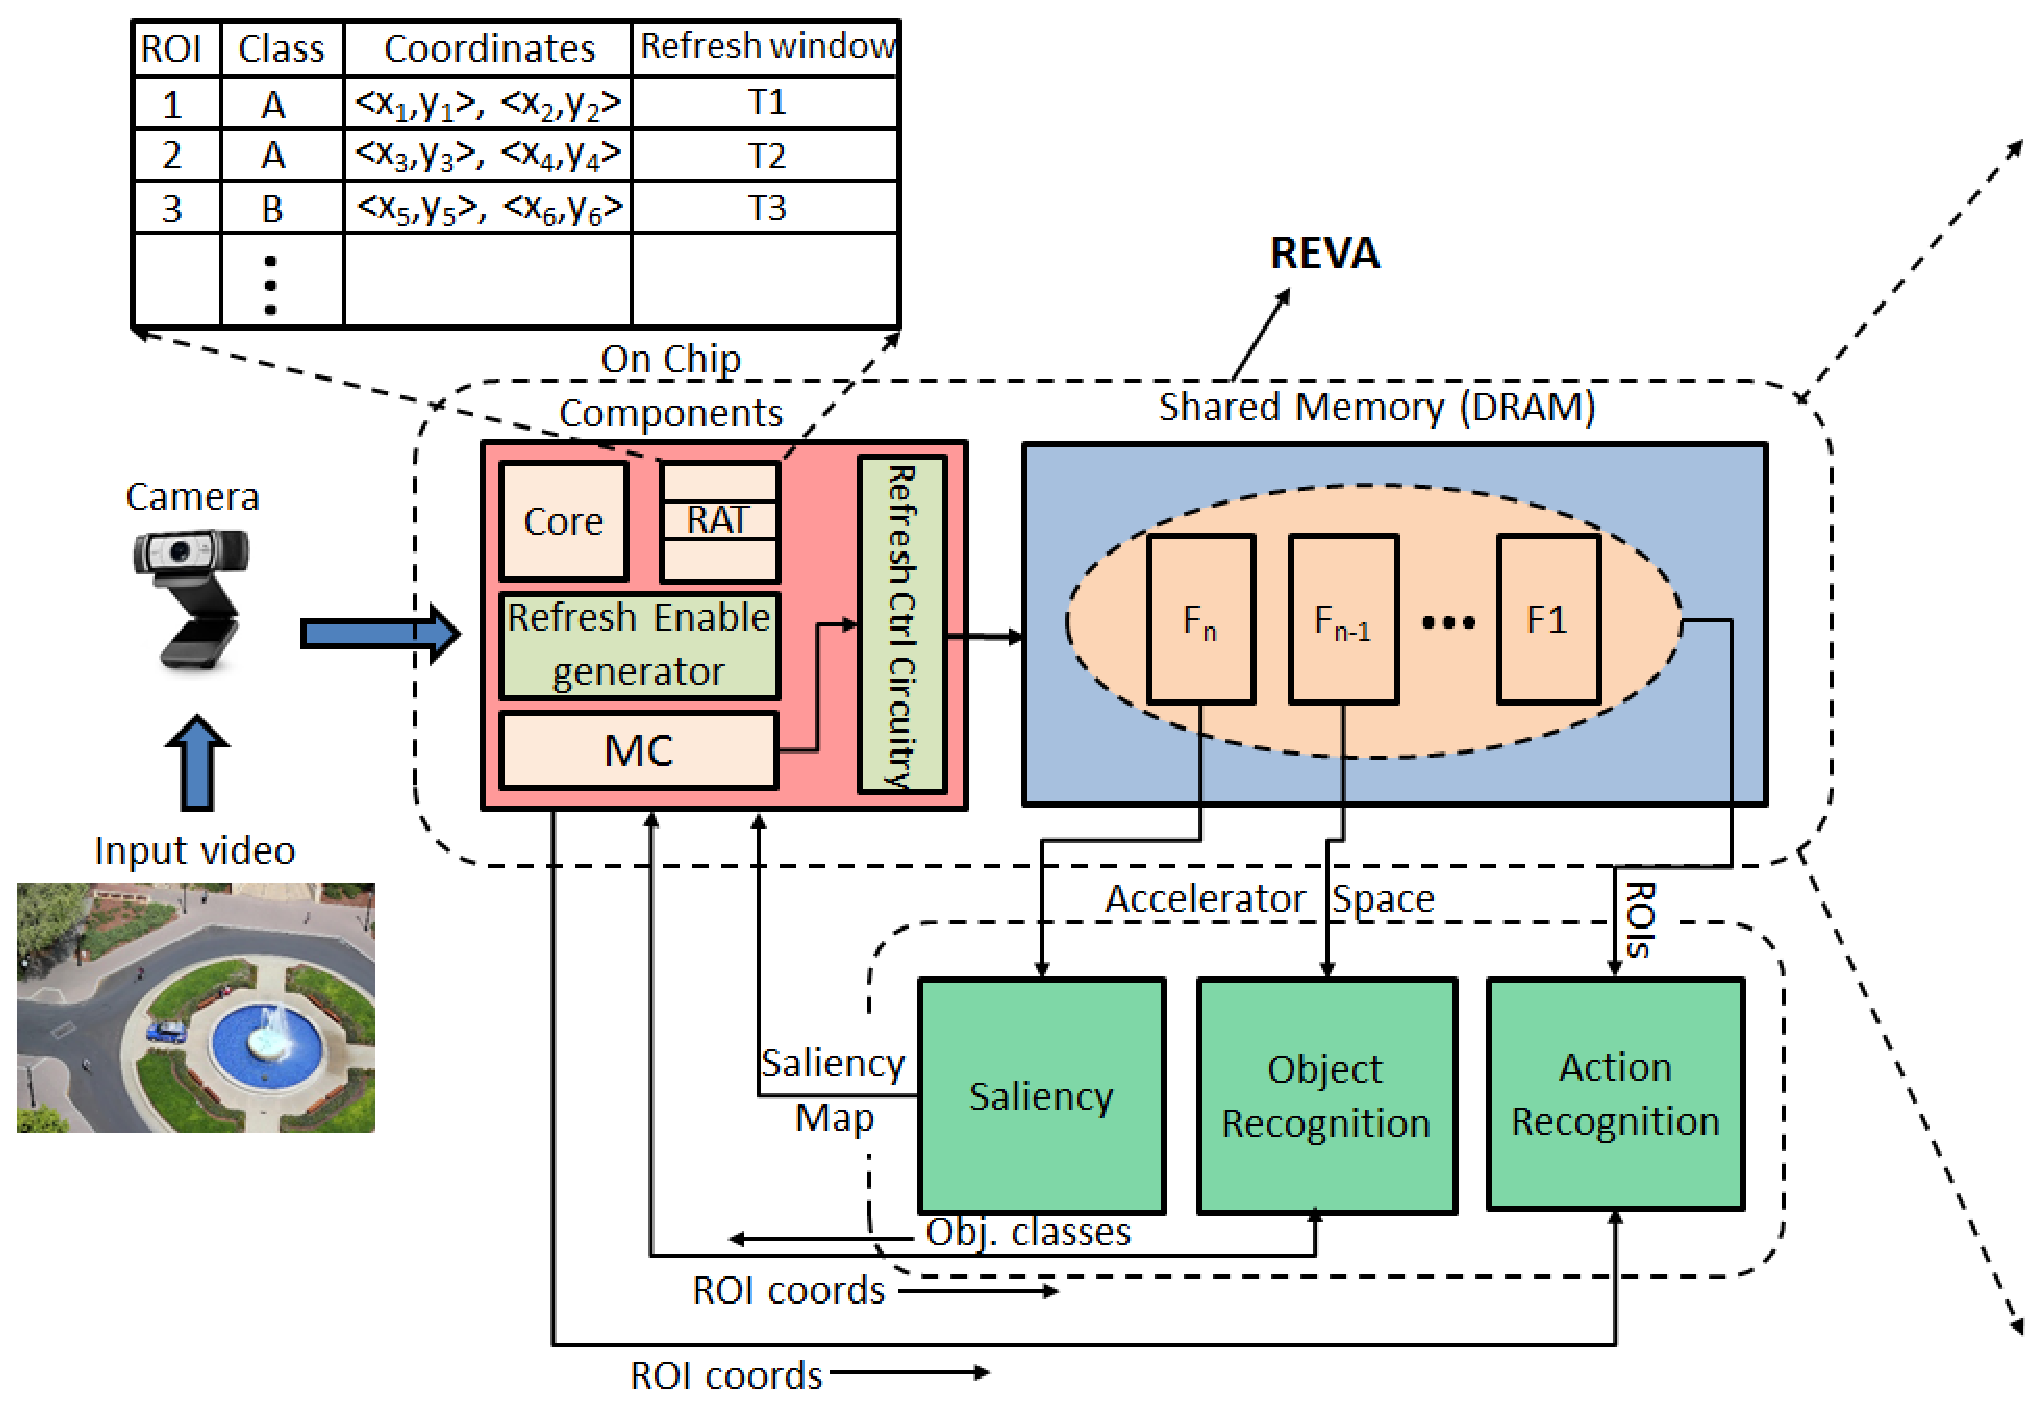
\epsfig{file=figs/reva_arch.eps, angle=0, width=0.95\linewidth, clip=}
\caption{\label{fig:reva}b) Architecture of Proposed System}
\end{minipage}
\begin{minipage}[b]{0.3\linewidth}
\raggedright
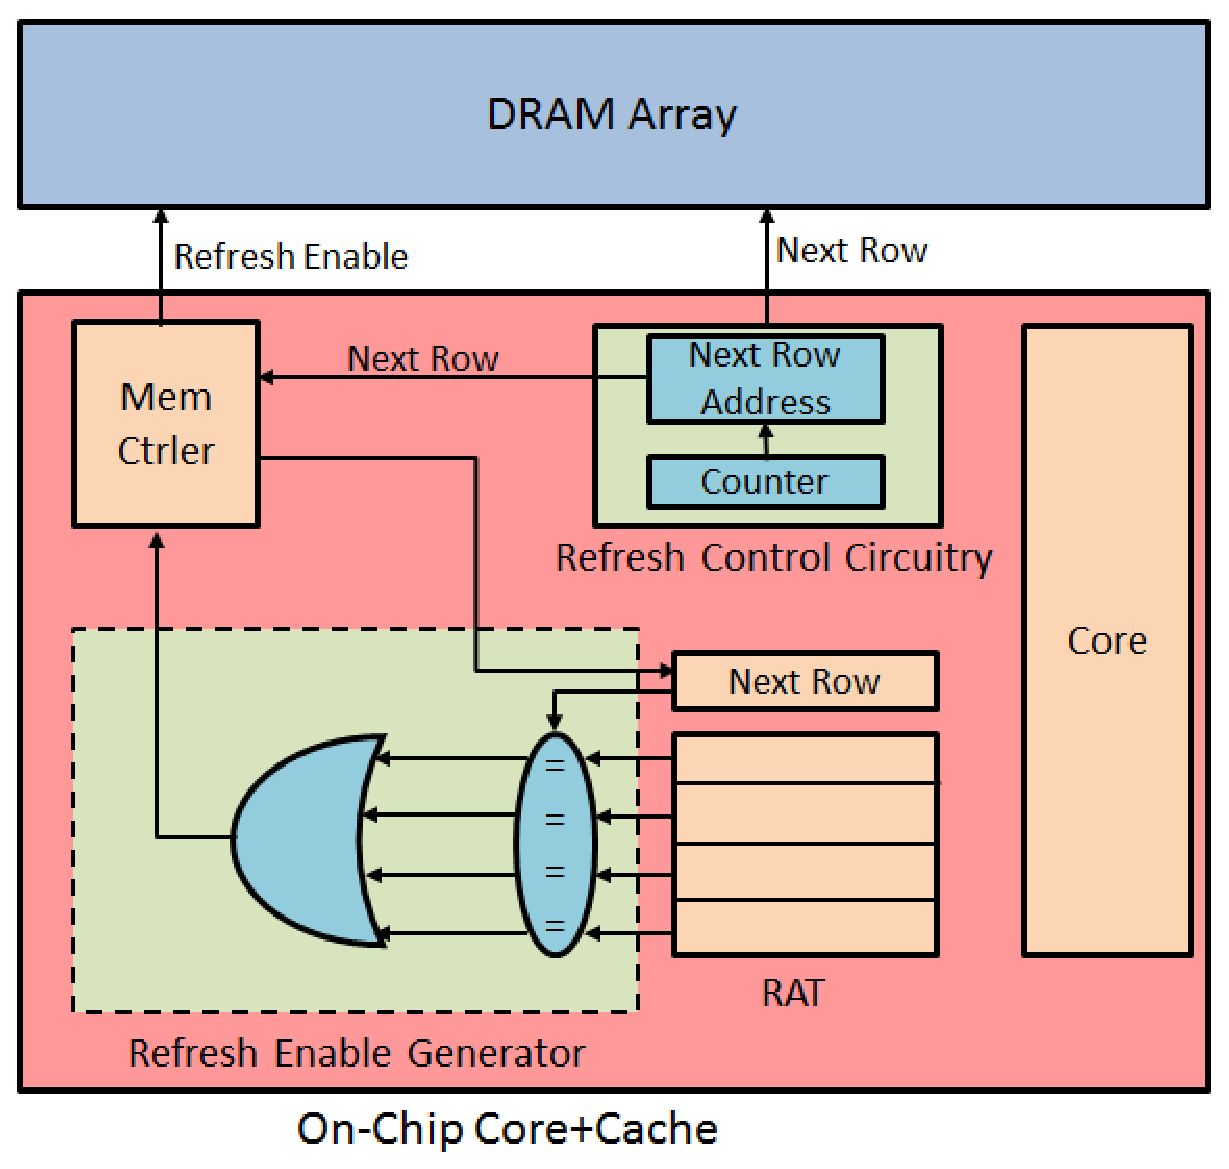
\epsfig{file=figs/refresh_circuitry.eps, angle=0, width=0.95\linewidth, clip=}
\caption{\label{fig:reva}c) Architecture of Proposed System}
\end{minipage}
\end{figure*}

\subsection{Differential Refresh Architecture}
As explained above, in the time duration of Refresh Cycle Time ($T_{RFC}$), a group of rows is refreshed sequentially when a refresh pulse is scheduled. A refresh pulse is sent every Refresh Interval ($T_{ref}$) time period.  When a refresh is scheduled, we keep track of the next row to be refreshed in a bank in the Next\_Row\_Address register. At the end of every refresh iteration, the content of this register is sent to the memory controller. At the memory controller, we maintain a CAM structure, RoI Address Table (RAT) to list Regions of Interest in each frame and their corresponding starting addresses. When the address of the next row to be refreshed does not match an RoI address on associative search, Refresh Enable signal is set to 0. This ensures that rows of an image in a bank that do not belong to RoIs are refreshed less frequently than the rows that contain Regions of Interest. We propose two schemes to support differential Refresh rates across different sections of an image. 

Each image frame is interleaved across banks at page granularity utilizing Row Buffer Locality. The saliency accelerator computes RoIs and updates the RAT,(figure xx) which is forwarded to the memory controller. After a refresh iteration, when the memory controller gets the Next\_Row\_Address and a match for this is found in the RAT, a refresh pulse is sent to the command queue; otherwise Refresh Enable signal is set to low. An RoI is a 2-d rectangular tile and might correspond to different rows in different banks; the group of rows containing a portion of the RoI might also have non-RoI regions striped across multiple banks. Still, the energy overhead of refreshing non-RoI regions in rows that contain RoI is x\% lesser than the energy overhead incurred on applying a uniform auto-refresh policy to the entire image. Since the non-RoI regions of the image are not subsequently read/written to, we allow the non-critical sections of the image to degrade with infrequent refreshes.  

It needs to be noted that for a completely stream based processing, where there is a single-pass streaming access of the image, a no-refresh policy needs to implemented for the entire image allowing corruption. Since a read operation inherently involves a refresh and each image row is read no more than once, this necessitates a no-refresh policy. 

This scheme involves communication overhead between memory controller and the refresh controller since the address of the next row to be refreshed is sent after every refresh iteration. An alternative would be to assign fixed refresh rates for different sections of a bank. For example, the upper addresses of a bank can be configured for no refresh and the lower addresses for auto-refresh policy. However this would involve mapping the physical pages of a Region of Interest to a specific partition in the bank incurring additional OS overhead and the scheme we propose does not involve page-level mapping of Virtual Addresses of RoIs to physical pages of a partition. Also, when the saliency accelerator generates the saliency map, RoIs are not written to dedicated variable refresh frequency partitions again. Instead the saliency map computed is used to derive RoIs in input image already stored in memory and refresh frequencies are varied based on the location of RoIs. 



